\section{Network Server Configuration}

\subsection{Node definition}

The \gls{LoRaWAN} end-node is registered within the ResIoT platform under the name \textbf{SN\_NODE\_J}. To ensure secure and unique connectivity within the network, the device is configured using the \gls{OTAA} method. Its primary identifiers include:

\begin{itemize}
    \item \textbf{Device EUI:} 7a:39:32:35:59:37:91:94.
    \item \textbf{Application EUI:} SEN\_NET\_2526.
    \item \textbf{Application KEY:} f3:1c:2e:8b:c6:71:28:1d:51:16:f0:8f:f0:b7:92:8f.
\end{itemize}

The node is set as a \gls{LoRaWAN} Class A device, operating on the EU868 frequency band. The internal data architecture of the node is organized through a series of \textbf{Node Fields} that act as the destination for the decoded payload values, defined in \autoref{tab:node_fields}.

\begin{table}[h]
    \centering
    \caption{Node Field Definitions for SN\_NODE\_J}
    \label{tab:node_fields}
    \begin{tabular}{p{0.2\textwidth}p{0.16\textwidth}p{0.05\textwidth}p{0.12\textwidth}p{0.16\textwidth}}
        \toprule
        \textbf{Field Tag} & \textbf{Content Type} & & \textbf{Field Tag} & \textbf{Content Type} \\ 
        \midrule
        Light & Numeric & & Latitude & Numeric \\ 
        Moisture & Numeric & & Longitude & Numeric \\ 
        Temperature & Numeric & & Altitude & Numeric \\ 
        Humidity & Numeric & & Time & String \\ 
        Red / Green / Blue & Numeric & & Sats & Numeric \\ 
        X / Y / Z & Numeric \\  
        \bottomrule
    \end{tabular}
\end{table}

\subsection{LUA Scripting}

The data transmitted by the end-node is received by the ResIoT platform as a hexadecimal payload. To make this information actionable, a LUA script is implemented to decode the raw byte array into human-readable sensor values. The script is structured into three main functional blocks:

\begin{itemize}
    \item \textbf{Binary Conversion Logic:} In \gls{LoRaWAN} payloads, data is sent in binary format. The function \texttt{bytesToInt} handles Little Endian conversion. It reconstructs integers by iterating through the byte array and applying the formula:
    \begin{equation}
        Value = \sum_{i=0}^{size-1} bytes[start + i] \cdot 256^i
    \end{equation}
    It also includes logic to handle signed integers using Two's Complement verification.

\begin{lstlisting}[language=lua, caption={LUA SN\_TEST\_J - Binary Conversion Logic}]
    -- Helper function to convert bytes to Integer (Little Endian)
    function bytesToInt(bytes, start, size, signed)
        local val = 0
        for i = 0, size - 1 do
            val = val + (bytes[start + i] * (256 ^ i))
        end
        if signed and val >= (256 ^ size) / 2 then
            val = val - (256 ^ size)
        end
        return val
    end
\end{lstlisting}

    \item \textbf{Payload Decapsulation:} The \texttt{parsePayload} function slices the buffer to extract specific sensor variables based on predefined offsets matching the \nameref{trama} subsection. Each variable is scaled according to its resolution and unit requirements.

\begin{lstlisting}[language=lua, caption={LUA SN\_TEST\_J - Payload Parsing}]
    function parsePayload(appeui, deveui, payload)
        -- Convert hex payload to byte array
        local bytes = resiot_hexdecode(payload)

        -- 1. GPS Data (1 to 17)
        local lat  = bytesToInt(bytes, 1, 4, true) / 1000000.0
        local lon  = bytesToInt(bytes, 5, 4, true) / 1000000.0
        local alt  = bytesToInt(bytes, 9, 4, true) / 100.0 

        -- GPS Time (13-15) HHMMSS
        local hh = bytes[13]
        local mm = bytes[14]
        local ss = bytes[15]
        local time = string.format("%02d:%02d:%02d", hh, mm, ss)

        local sats = bytes[16]                            

        -- 2. Temperature and Humidity Data (17 to 20)
        local temp = bytesToInt(bytes, 17, 2, true) / 100.0
        local hum  = bytesToInt(bytes, 19, 2, false) / 100.0

        -- 3. Brightness and Moisture (21 to 24)
        local light    = bytesToInt(bytes, 21, 2, false) / 10.0
        local moisture = bytesToInt(bytes, 23, 2, false) / 10.0

        -- 4. Color RGB (Offsets 25 to 27)
        local r = bytes[25]
        local g = bytes[26]
        local b = bytes[27]

        -- 5. Accelerometer (28 to 30)
        -- These are int8 (signed). If value > 127, it's negative.
        local function toInt8(b) return b > 127 and b - 256 or b end
        local x = toInt8(bytes[28]) / 10.0
        local y = toInt8(bytes[29]) / 10.0
        local z = toInt8(bytes[30]) / 10.0

        ...
    end
\end{lstlisting}

    \item \textbf{Platform Integration:} After decoding, the script utilizes the \texttt{resiot\_setnodevalue} function. This updates the device within the platform, mapping the decoded variables to specific node fields. Also, debug logs are generated to facilitate monitoring and troubleshooting.

\begin{lstlisting}[language=lua, caption={LUA SN\_TEST\_J - Debug and Node Update}]
    function parsePayload(appeui, deveui, payload)
        ...

        -- Debug Logs
        resiot_debug(string.format("GPS: Lat: %.6f, Long: %.6f, Alt: %.2f, Time: %s, Sats: %d", lat, lon, alt, time, sats))
        resiot_debug(string.format("Sensors: Temp: %.2f, Hum: %.2f, Light: %.1f, Moisture: %.1f", temp, hum, light, moisture))
        resiot_debug(string.format("Color: R:%d, G:%d, B:%d", r, g, b))
        resiot_debug(string.format("Accel: X:%.1f, Y:%.1f, Z:%.1f", x, y, z))

        -- Update Nodes in ResIoT
        resiot_setnodevalue(appeui, deveui, "Latitude", lat)
        resiot_setnodevalue(appeui, deveui, "Longitude", lon)
        resiot_setnodevalue(appeui, deveui, "Altitude", alt)
        resiot_setnodevalue(appeui, deveui, "Time", time)
        resiot_setnodevalue(appeui, deveui, "Sats", sats)
        resiot_setnodevalue(appeui, deveui, "Temperature", temp)
        resiot_setnodevalue(appeui, deveui, "Humidity", hum)
        resiot_setnodevalue(appeui, deveui, "Light", light)
        resiot_setnodevalue(appeui, deveui, "Moisture", moisture)
        resiot_setnodevalue(appeui, deveui, "Red", r)
        resiot_setnodevalue(appeui, deveui, "Green", g)
        resiot_setnodevalue(appeui, deveui, "Blue", b)
        resiot_setnodevalue(appeui, deveui, "X", x)
        resiot_setnodevalue(appeui, deveui, "Y", y)
        resiot_setnodevalue(appeui, deveui, "Z", z)
    end
\end{lstlisting}

    \item \textbf{Manual Testing:} The script also includes an \texttt{Origin} check, allowing for manual testing with a static hex string or automatic processing when a live uplink is detected from the \gls{LoRaWAN} gateway.

\begin{lstlisting}[language=lua, caption={LUA SN\_TEST\_J} - Manual Testing Block]
    -- --- Main Process ---
    Origin = resiot_startfrom()

    if Origin == "Manual" then
        -- Test payload (30 bytes hex)
        payload = "010203040506070809101112131415161718192021222324252627282930" 
        appeui = "70b3d57ed000fc4d"
        deveui = "7a39323559379194"
    else
        appeui = resiot_comm_getparam("appeui")
        deveui = resiot_comm_getparam("deveui")
        payload, err = resiot_getlastpayload(appeui, deveui)
    end

    parsePayload(appeui, deveui, payload)
\end{lstlisting}

\end{itemize}

The LUA script is integrated into the ResIoT ecosystem through the \gls{LoRaWAN} node's automation logic. Rather than running as a static process, the code is embedded within the \textbf{On RX} (On Receive) event. This configuration establishes an event-driven architecture where the script remains idle until a new radio frame is successfully demodulated by the gateway and forwarded to the network server.

\begin{figure}[H]
    \centering
    \includegraphics[width=0.7\textwidth]{images/scene.png}
    \caption{ResIoT Node Automation - On RX Event}
    \label{fig:scene}
\end{figure}

Once an uplink packet is received, the platform automatically triggers the execution of the script, passing the device identifiers and the raw hexadecimal payload as input parameters.

\subsection{Dashboard}

The monitoring interface is organized within a dedicated group named \textbf{SN\_GROUP\_J}. The dashboard consists of a variety of widgets. The following list details the specific widgets and their respective visualization types:

\begin{itemize}
    \item \textbf{Node J - Temperature / Humidity / Brightness / Soil Moisture:} These environmental parameters are displayed using \textbf{Gauge} widgets.
    \item \textbf{Node J - Historical Values:} A \textbf{Line Chart} is dedicated to tracking the temporal evolution of sensor data over time.
    \item \textbf{Node J - Alarms:} A \textbf{Table Values} widget is configured to show the status of the boolean alarm flags, allowing for quick identification of threshold breaches (Temperature / Humidity / Brightness / Soil Moisture).
    \item \textbf{Node J - Leaf Color:} The \gls{RGB} values are represented through a \textbf{Pie chart} widget.
    \item \textbf{Node J - Acceleration ($m/s^2$):} Acceleration data is visualized using a \textbf{Line Chart}.
    \item \textbf{Node J - Location:} A \textbf{Maps} widget is used to track the \gls{GPS} data.
\end{itemize}

\begin{figure}[H]
    \centering
    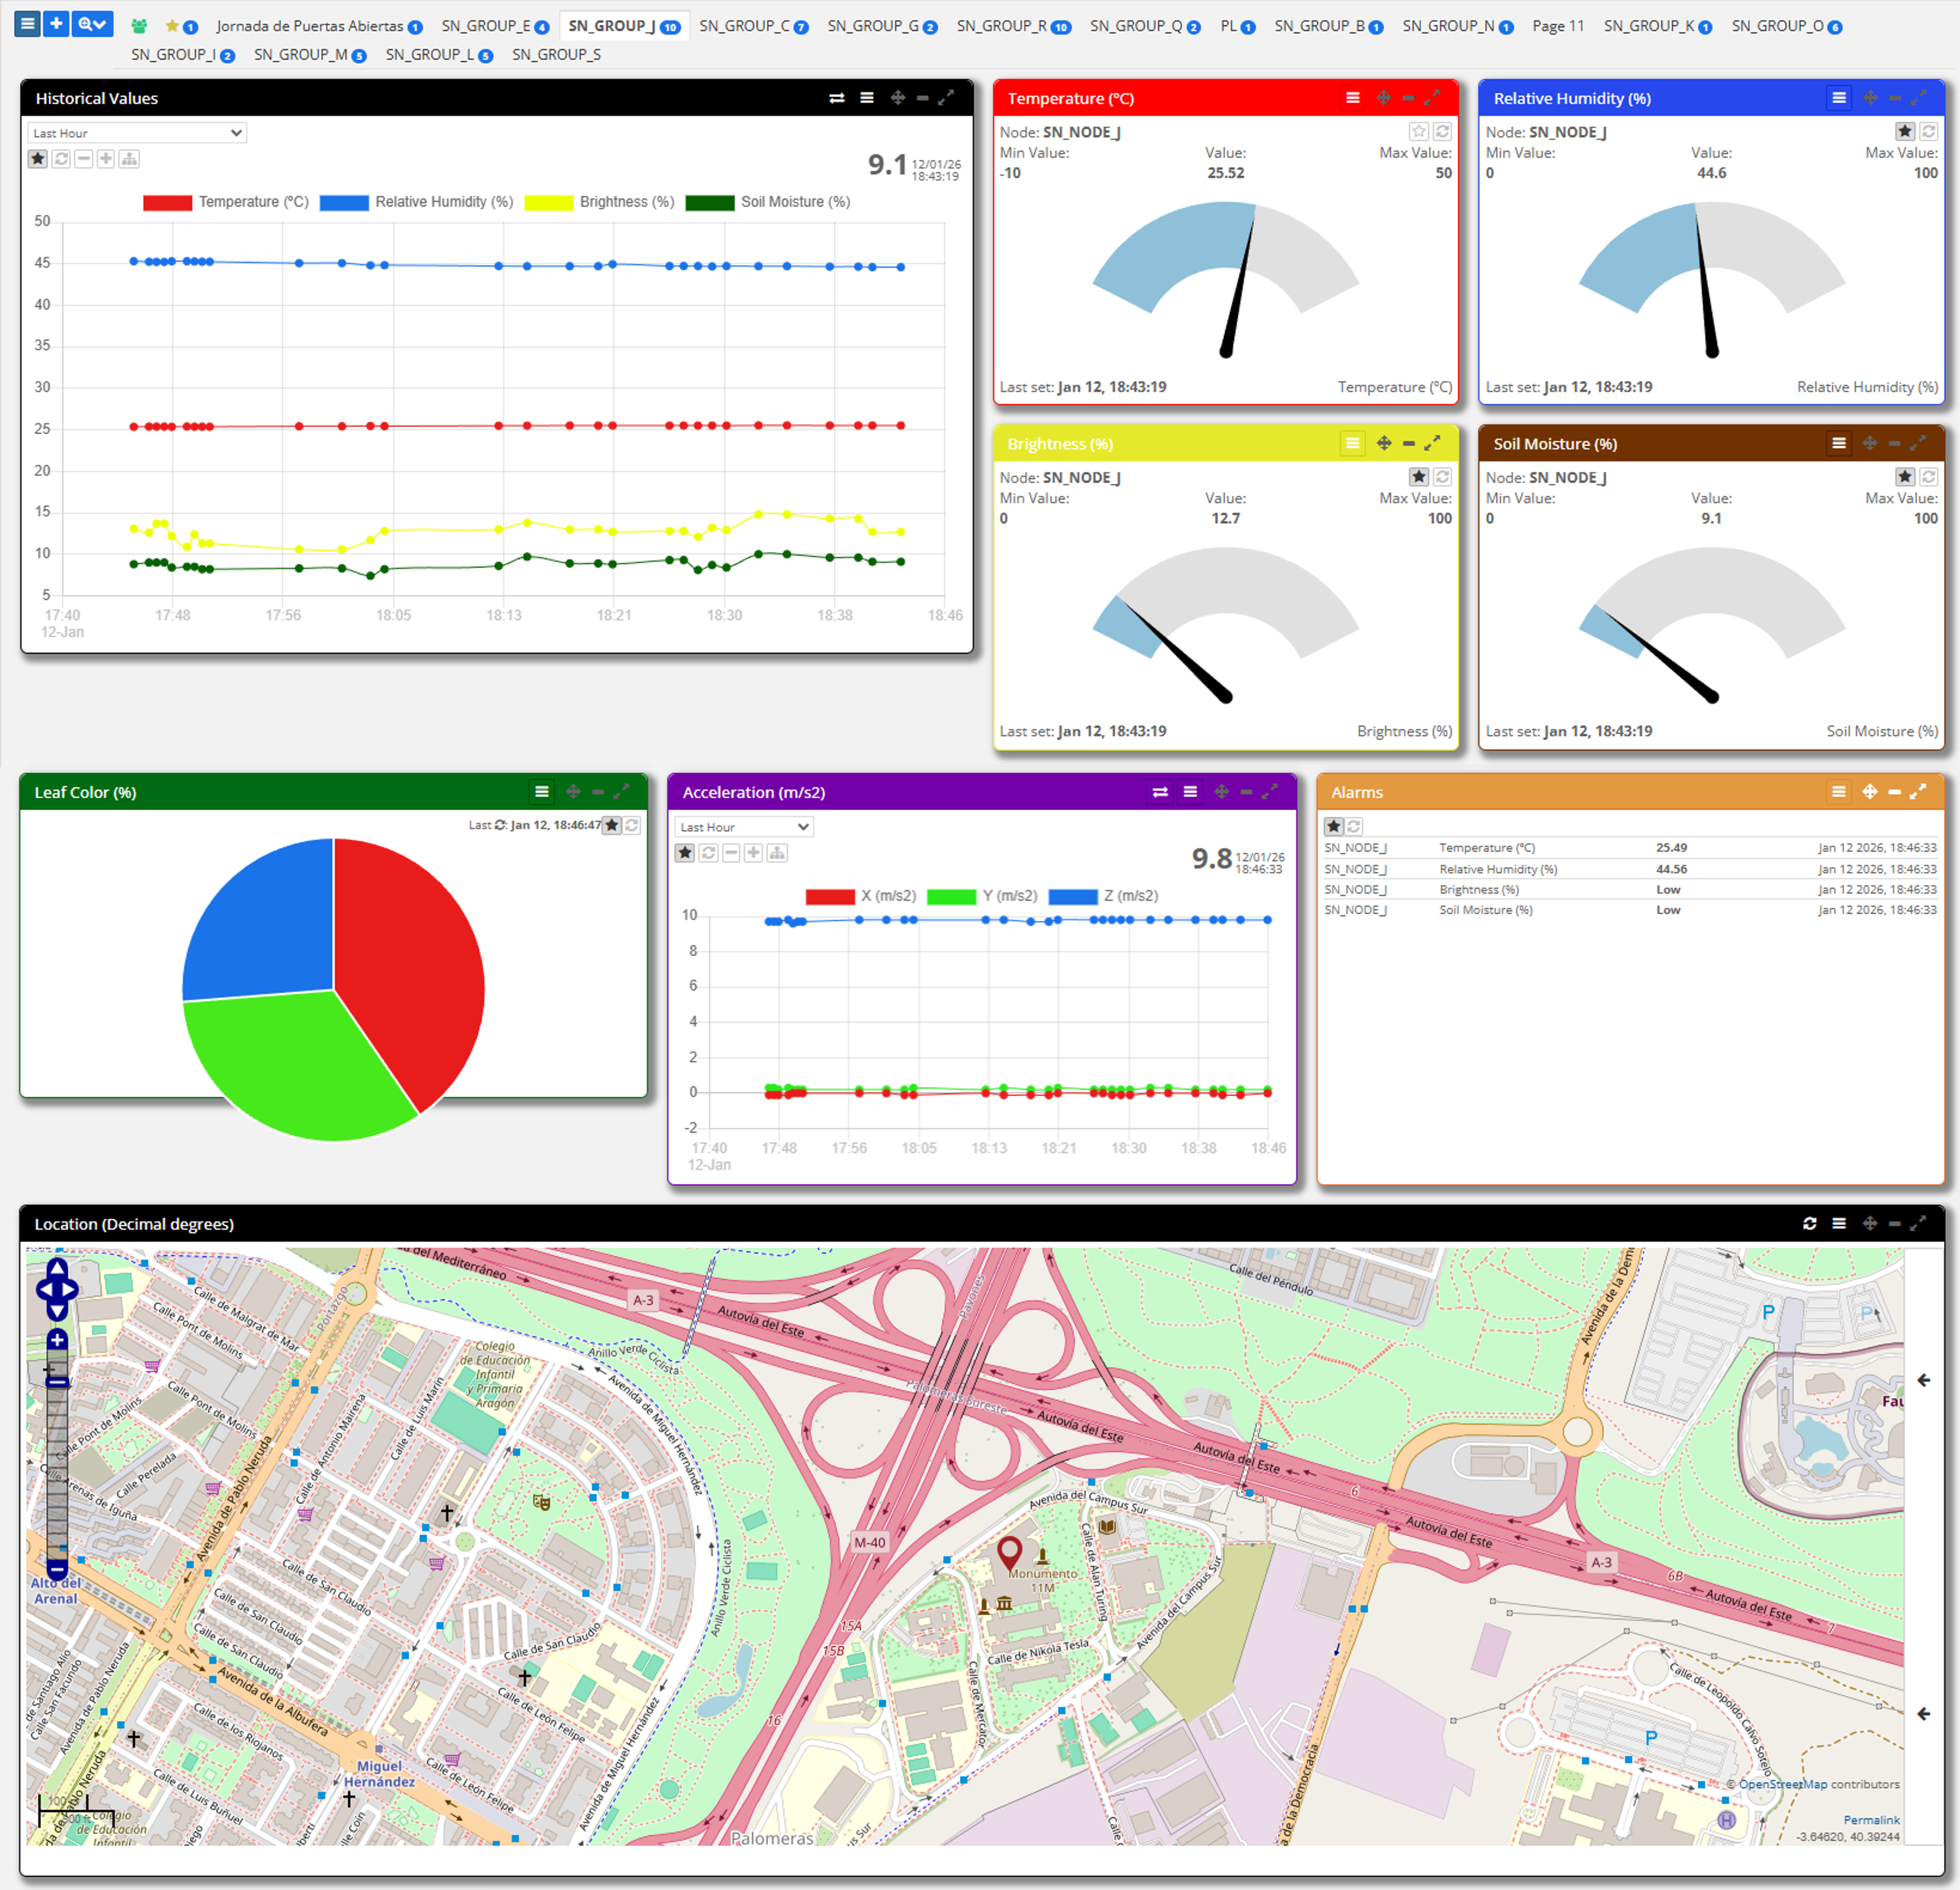
\includegraphics[width=1\textwidth]{images/dashboard.png}
    \caption{ResIoT Dashboard - SN\_GROUP\_J}
    \label{fig:dashboard}
\end{figure}

\subsubsection{Temperature / Humidity / Brightness / Soil Moisture Gauges}

The primary environmental metrics are visualized through four specialized \textbf{Gauge} widgets. The configuration for these gauges (as exemplified by the Temperature widget in Figure \ref{fig:gauge_conf}) is defined by the following parameters:

\begin{itemize}
    \item \textbf{Data Mapping:} Each widget is linked to the specific numeric \texttt{Node Field} updated by the LUA script.
    \item \textbf{Range Calibration:} To provide context to the raw data, specific minimum and maximum thresholds are established:
    \begin{itemize}
        \item \textbf{Temperature:} Set from -10°C to 50°C.
        \item \textbf{Humidity / Brightness / Soil Moisture:} Calibrated on a percentage scale.
    \end{itemize}
    \item \textbf{Visual Styling:} Each gauge utilizes a distinct header color.
    \item \textbf{Unit Management:} The widgets are configured with their respective Units of Measurement.
    \item \textbf{Refresh Logic:} The chart includes an \textbf{Autorefresh} feature, ensuring the visualization remains synchronized with the latest environmental data processed by the platform.
\end{itemize}

\begin{figure}[H]
    \centering
    \includegraphics[width=1\textwidth]{images/gauge_temp.png}
    \caption{Gauge Configuration - Temperature Example}
    \label{fig:gauge_conf}
\end{figure}

As shown in Figure \ref{fig:gauges}, the gauges also display the timestamp of the last received data packet (\textbf{"Last set"}), confirming the real-time nature of the \textbf{On RX} automation process.

\begin{figure}[H]
    \centering
    \includegraphics[width=0.8\textwidth]{images/gauges.png}
    \caption{ResIoT Dashboard - Temperature / Humidity / Brightness / Soil Moisture Gauges}
    \label{fig:gauges}
\end{figure}

\subsubsection{Historical Values}

The \textbf{Node J - Historical Values} widget is a \textbf{Line Chart} designed to monitor the temporal evolution of the environment.

\begin{figure}[H]
    \centering
    \includegraphics[width=0.8\textwidth]{images/historical.png}
    \caption{ResIoT Dashboard - Historical Values Line Chart}
    \label{fig:historical}
\end{figure}

The configuration of this chart, as illustrated in Figure \ref{fig:hist_conf}, is based on the following technical parameters:

\begin{itemize}
    \item \textbf{Data Aggregation:} The chart simultaneously plots four distinct data series from the \texttt{SN\_NODE\_J} node fields.
    \item \textbf{Color Coding:} Specific colors are assigned to each variable.
    \item \textbf{Time Window:} The widget is configured with a \textbf{Last Hour} default interval.
    \item \textbf{Dynamic Scaling:} The Y-axis automatically adjusts to the numeric range of the incoming data, while the X-axis represents the chronological timeline updated by the \texttt{On RX} automation.
    \item \textbf{Refresh Logic}.
\end{itemize}

\begin{figure}[H]
    \centering
    \includegraphics[width=1\textwidth]{images/historical_conf.png}
    \caption{Line Chart Configuration - Historical Values}
    \label{fig:hist_conf}
\end{figure}


\subsubsection{Alarms}

The \textbf{Node J - Alarms} widget is implemented as a \textbf{Table Values} display. Unlike the gauges, which show raw numerical data, this table is specifically configured to interpret threshold breaches and translate them into human-readable alerts.

\begin{figure}[H]
    \centering
    \includegraphics[width=0.9\textwidth]{images/alarms.png}
    \caption{ResIoT Dashboard - Alarms Table}
    \label{fig:alarms}
\end{figure}

As illustrated in the configuration details in Figure \ref{fig:alarms_conf}, the widget utilizes a conditional string replacement logic to define the status of each variable:

\begin{itemize}
    \item \textbf{Temperature Logic:} The system monitors for extreme conditions, displaying \textbf{"High"} if the value exceeds $50$ and \textbf{"Low"} if it falls below $-10$.
    \item \textbf{Percentage Thresholds:} For Relative Humidity, Brightness, and Soil Moisture, a unified logic is applied where values above $75$ trigger a \textbf{"High"} status and values below $25$ trigger a \textbf{"Low"} status.
    \item \textbf{Real-time Monitoring:} If the current values are within the safe operational range, the table displays the actual numerical value.
    \item \textbf{Data Synchronization:} Every entry in the table is accompanied by a timestamp (\texttt{"Date Last Setting"}), ensuring that the alerts correspond to the most recent \gls{LoRaWAN} uplink processed by the \texttt{On RX} automation.
    \item \textbf{Refresh Logic}.
\end{itemize}

\begin{figure}[H]
    \centering
    \includegraphics[width=0.9\textwidth]{images/alarms_conf.png}
    \caption{Table Configuration}
    \label{fig:alarms_conf}
\end{figure}


\subsubsection{Leaf Color}

The \textbf{Node J - Leaf Color} widget provides a qualitative representation of \gls{RGB} color data using a \textbf{Pie Chart} format.

\begin{figure}[H]
    \centering
    \includegraphics[width=0.8\textwidth]{images/color.png}
    \caption{ResIoT Dashboard - Leaf Color Pie Chart}
    \label{fig:color}
\end{figure}

The configuration of this widget, as detailed in Figure \ref{fig:color_conf}, includes the following parameters:

\begin{itemize}
    \item \textbf{Data Integration:} The chart aggregates the three colors.
    \item \textbf{Visual Mapping:} Red for the Red (\%) field, Green for the Green (\%) field, and Blue for the Blue (\%) field.
    \item \textbf{Interactive Display:} The widget is configured to show specific values upon user interaction.
    \item \textbf{Refresh Logic}.
\end{itemize}

\begin{figure}[H]
    \centering
    \includegraphics[width=1\textwidth]{images/color_conf.png}
    \caption{Pie Chart Configuration}
    \label{fig:color_conf}
\end{figure}

\clearpage

\subsubsection{Acceleration}

Acceleration monitoring is performed through the \textbf{Node J - Acceleration ($m/s^2$)} widget, which utilizes a \textbf{Line Chart}. 

\begin{figure}[H]
    \centering
    \includegraphics[width=0.8\textwidth]{images/accel.png}
    \caption{ResIoT Dashboard - Acceleration Line Chart}
    \label{fig:accel}
\end{figure}

The implementation for this chart is defined by the following configuration parameters:

\begin{itemize}
    \item \textbf{Axis Mapping:} The X, Y and Z fields are updated as signed integers by the LUA script to reflect directional acceleration.
    \item \textbf{Visual Representation:} The chart uses a standardized color coding scheme: Red for the \textbf{X-axis}, Green for the \textbf{Y-axis}, and Blue for the \textbf{Z-axis}.
    \item \textbf{Data Interval:} The widget is configured with a \textbf{Last Hour} default interval.
    \item \textbf{Scaling and Units:} The Y-axis is scaled in meters per second squared ($m/s^2$).
    \item \textbf{Refresh Logic}.
\end{itemize}

\begin{figure}[H]
    \centering
    \includegraphics[width=1\textwidth]{images/accel_conf.png}
    \caption{Line Chart Configuration - Acceleration}
    \label{fig:accel_conf}
\end{figure}

\subsubsection{Location}

Geospatial monitoring is provided through the \textbf{Node J - Location} widget, which integrates GPS data into an interactive mapping interface.

\begin{figure}[H]
    \centering
    \includegraphics[width=0.9\textwidth]{images/location.png}
    \caption{ResIoT Dashboard - Location Map}
    \label{fig:location}
\end{figure}

The technical implementation of the location system is based on the following configurations:

\begin{itemize}
    \item \textbf{Spatial Data Mapping:} As shown in Figure \ref{fig:location_conf}, the widget is linked to five critical node fields: \texttt{Latitude}, \texttt{Longitude}, \texttt{Altitude}, \texttt{Time}, and \texttt{Sats} (Satellite count).
\end{itemize}

\begin{figure}[H]
    \centering
    \includegraphics[width=0.9\textwidth]{images/location_conf.png}
    \caption{Map Configuration - Location}
    \label{fig:location_conf}
\end{figure}

Clicking on the specific red location pin (as shown in \autoref{fig:location_info}) triggers a pop-up window, that provides the latitude, longitude, altitude, the exact time of the record, and the satellite count.

\begin{figure}[H]
    \centering
    \includegraphics[width=1\textwidth]{images/location_info.png}
    \caption{ResIoT Dashboard - Location Info}
    \label{fig:location_info}
\end{figure}

